\section{Arquitectura y diseño territorial de la red}
\label{sec:arquitectura}

\subsection{Diagrama general}
\label{sec:diagrama_general}
La \autoref{fig:diagrama_general} representa la red desde el proveedor mayorista hasta el abonado. La red de distribución óptica (ODN, \textit{Optical Distribution Network}) es la parte pasiva comprendida entre la interfaz óptica del puerto PON de la OLT y la interfaz óptica de la ONT \cite{g984_2}. Incluye los patch cords y el ODF del hub, los cables, las cajas de empalme, los splitters, las cajas terminales, la acometida y la roseta del abonado. Los equipos activos (OLT y ONT) quedan fuera de la ODN.

\begin{figure}[H]
    \centering
    \resizebox{\textwidth}{!}{%
    \begin{tikzpicture}[font=\footnotesize, node distance=0.5cm,
        activo/.style={draw, thick, rounded corners=2pt, fill=blue!10, minimum height=1.1cm, align=center, text width=2.1cm},
        pasivo/.style={draw, thick, fill=gray!10, minimum height=1.1cm, align=center, text width=2.1cm},
        caja/.style={draw, thick, rounded corners=5pt, fill=orange!15, minimum height=1.1cm, align=center, text width=2.1cm},
        flecha/.style={-{Stealth}, thick}]
        % Fila superior: transporte y hub
        \node[activo] (refefo) at (0,3.2) {\textbf{Nodo REFEFO}\\ARSAT\\Marcos Juárez};
        \node[activo] (router) at (4.2,3.2) {\textbf{Router de borde}\\BNG, cachés};
        \node[activo] (sw) at (7.6,3.2) {\textbf{Switch de}\\\textbf{agregación}\\$10 \, [GE]$};
        \node[activo] (olt) at (11.0,3.2) {\textbf{OLT}\\VSOL V1600G2-B\\SFP Clase C+};
        \node[pasivo] (odf) at (14.4,3.2) {\textbf{ODF}\\DIO B144\\SC/APC};
        \draw[flecha] (refefo) -- node[above, font=\scriptsize]{Enlace P2P} node[below, font=\scriptsize]{10GBASE-LR} (router);
        \draw[flecha] (router) -- (sw);
        \draw[flecha] (sw) -- node[above, font=\scriptsize]{LAG $2 \times 10G$} (olt);
        \draw[flecha] (olt) -- node[above, font=\scriptsize]{patch cord} (odf);
        % Fila inferior: planta externa
        \node[caja] (ceo) at (14.4,0) {\textbf{CEO de cluster}\\FK-CEO-4M\\(derivación)};
        \node[caja] (cd) at (11.0,0) {\textbf{Caja de}\\\textbf{distribución}\\splitter 1:4};
        \node[caja] (cto) at (7.6,0) {\textbf{CTO}\\FK-CTO-16MC\\splitter 1:16};
        \node[pasivo] (roseta) at (4.2,0) {\textbf{Roseta}\\óptica\\SC/APC};
        \node[activo] (ont) at (0,0) {\textbf{ONT}\\VSOL V2802RH};
        \draw[flecha] (odf) -- node[right, font=\scriptsize, align=left]{Troncal\\AS80-S TS\\24 a 144 F} (ceo);
        \draw[flecha] (ceo) -- node[above, font=\scriptsize]{Cable de cluster} node[below, font=\scriptsize]{MINI-RA 24 F} (cd);
        \draw[flecha] (cd) -- node[above, font=\scriptsize]{Distribución} node[below, font=\scriptsize]{MINI-RA 12 F} (cto);
        \draw[flecha] (cto) -- node[above, font=\scriptsize]{Drop} node[below, font=\scriptsize]{Fig.8 G.657.A} (roseta);
        \draw[flecha] (roseta) -- node[above, font=\scriptsize]{patch cord} (ont);
        % Límite de la ODN
        \draw[very thick, dashed, red!70!black, rounded corners=8pt] (12.55,4.3) -- (16.1,4.3) -- (16.1,-1.2) -- (1.75,-1.2) -- (1.75,1.05) -- (12.55,1.05) -- cycle;
        \node[red!70!black, font=\small\bfseries] at (8.6,1.35) {ODN (red de distribución óptica pasiva)};
        % Referencias de sitio
        \node[font=\scriptsize, gray] at (9.3,4.4) {Hub COYSPU (9 de Julio 99)};
        \node[font=\scriptsize, gray] at (0,-1.0) {Domicilio};
        \node[font=\scriptsize, gray] at (0,4.4) {Proveedor mayorista};
    \end{tikzpicture}%
    }
    \caption{Diagrama general de la red: desde el proveedor mayorista hasta el abonado. La línea de trazos delimita la ODN.}
    \label{fig:diagrama_general}
\end{figure}

La división se realiza en dos niveles: un splitter 1:4 en la caja de distribución de cada sector y un splitter 1:16 en cada caja terminal. La relación total es de 1:64 por puerto PON. Se eligió división distribuida en dos niveles porque reduce la cantidad de fibras del troncal (una por sector en lugar de una por caja terminal) y permite ubicar la caja terminal a pocos metros de las viviendas.

\subsection{Organización del área de cobertura}
\label{sec:organizacion}
El hub (nodo cabecera) se ubica en la sede de la Cooperativa COYSPU, en 9 de Julio 99, Marcos Juárez. Allí se instalan la OLT, el ODF, el equipamiento de borde y la terminación del enlace mayorista. El área se organiza en cuatro niveles jerárquicos:

\begin{table}[H]
    \centering
    \footnotesize
    \caption{Unidades de diseño y su relación.}
    \label{tab:unidades}
    \begin{tabular}{|l|p{6.4cm}|p{5.0cm}|}
        \hline
        \textbf{Unidad} & \textbf{Definición} & \textbf{Capacidad prevista} \\
        \hline
        Región & Mitad del área de cobertura a cada lado de la RP12 & Este: $6.153$ viviendas, 12 clusters, 92 sectores \\
        \hline
        Cluster & Grupo contiguo de hasta 8 sectores alimentado por un bloque de 24 fibras del troncal, que se deriva en una caja de empalme (CEO) & 7 u 8 sectores: entre 439 y 540 viviendas \\
        \hline
        Sector de diseño & Zona atendida por un puerto PON: un splitter 1:4 en su caja de distribución y hasta 4 CTO 1:16 & Hasta 68 viviendas, 64 salidas: 61 abonados al 90\,\% \\
        \hline
        Área de CTO & Grupo de viviendas atendido por una caja terminal & Hasta 17 viviendas, 16 salidas \\
        \hline
    \end{tabular}
\end{table}

\textbf{Metodología de sectorización.} Las viviendas de cada manzana se representan como puntos sobre su perímetro (\autoref{sec:casas}). Sobre ellos se aplica el siguiente procedimiento, implementado en Python con los datos de calles de OpenStreetMap:
\begin{enumerate}
    \item Se identifican los grupos de viviendas conexos, separados entre sí por más de $100 \, [m]$, para que ningún sector abarque zonas sin viviendas. En la Región Este resultan tres grupos: el casco urbano ($6.074$ viviendas) y dos barrios aislados al noreste (45 y 34 viviendas).
    \item Cada grupo se divide por bisecciones sucesivas en sectores contiguos de hasta 68 viviendas.
    \item Dentro de cada sector, las viviendas se asignan a hasta 4 CTO con capacidad de 17. Cada CTO se ubica en la esquina que minimiza la longitud de acometida más larga.
    \item Los sectores se agrupan en clusters contiguos de hasta 8 sectores.
\end{enumerate}

Resultan \textbf{12 clusters, 92 sectores y 365 cajas terminales} en la Región Este (\autoref{fig:sectores} y \autoref{tab:clusters}). Los 90 sectores del casco urbano tienen 4 CTO y entre 67 y 68 viviendas; los dos barrios aislados forman los sectores 91 (34 viviendas, 2 CTO) y 92 (45 viviendas, 3 CTO). El detalle de cada sector se presenta en el \autoref{anexo:sectores}.

\begin{figure}[H]
    \centering
    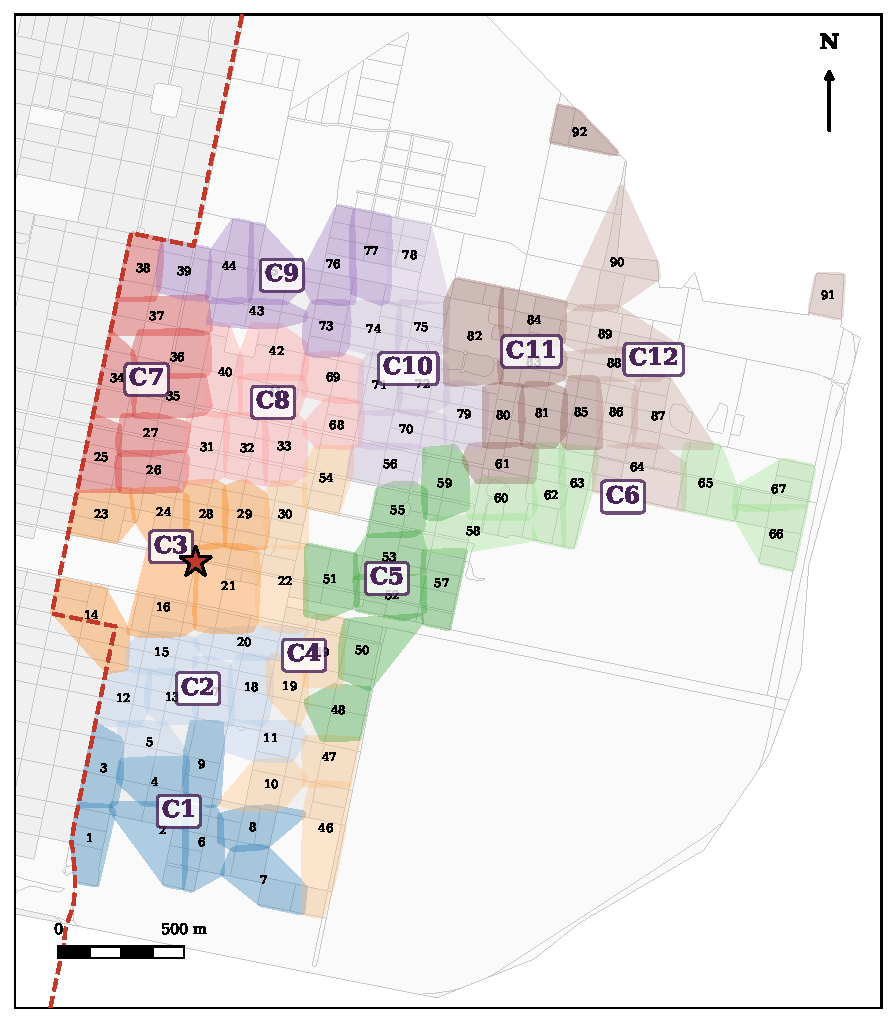
\includegraphics[width=0.95\textwidth]{plano_este_sectores.pdf}
    \caption{Región Este: clusters (C1 a C12) y sectores de diseño (1 a 92).}
    \label{fig:sectores}
\end{figure}

\begin{table}[H]\centering\footnotesize
\caption{Clusters de la Región Este: viviendas, abonados y longitudes.}\label{tab:clusters}
\setlength{\tabcolsep}{3pt}\begin{tabular}{|c|c|r|r|r|r|r|p{3.6cm}|}\hline \textbf{Cluster} & \textbf{Sect.} & \textbf{Viv.} & \textbf{Ab. 1.\textsuperscript{a} et.} & \textbf{Ab. final} & \textbf{L troncal [m]} & \textbf{Cable cl. [m]} & \textbf{Ubicación del CEO} \\ \hline
C1 & 8 & 540 & 243 & 486 & 909 & 1.683 & Avenida Zeballos y Perú \\ \hline
C2 & 8 & 540 & 243 & 486 & 388 & 1.857 & 3 de Febrero y Perú \\ \hline
C3 & 7 & 473 & 213 & 426 & 158 & 1.707 & 9 de Julio y Avenida San Martín \\ \hline
C4 & 8 & 540 & 243 & 486 & 474 & 3.444 & Champagnat y Pasaje Maipú \\ \hline
C5 & 8 & 540 & 243 & 486 & 674 & 2.713 & Boulevard Lardizabal y Garibaldi \\ \hline
C6 & 7 & 473 & 213 & 426 & 1.540 & 2.453 & Los Robles \\ \hline
C7 & 8 & 540 & 243 & 486 & 575 & 1.452 & Leandro N. Alem \\ \hline
C8 & 8 & 540 & 243 & 486 & 581 & 2.113 & Boulevard Hipólito Irigoyen y Justo José de Urquiza \\ \hline
C9 & 7 & 473 & 213 & 426 & 1.302 & 1.542 & 9 de Julio y Avenida Rivadavia \\ \hline
C10 & 8 & 538 & 243 & 485 & 1.317 & 1.811 & Bismark y O'Higgins \\ \hline
C11 & 8 & 517 & 233 & 466 & 1.857 & 2.861 & Avenida Roque Sanz Peña Este y Timoteo Gordillo \\ \hline
C12 & 7 & 439 & 198 & 396 & 2.566 & 2.613 & Hermanas Vicentinas y Pasaje Juan Cruz González Este \\ \hline
\textbf{Total} & \textbf{92} & \textbf{6.153} & \textbf{2.771} & \textbf{5.541} & \multicolumn{3}{l|}{} \\ \hline
\end{tabular}\end{table}


\subsection{Trazas generales}
\label{sec:trazas}
Los cables se tienden en forma aérea sobre la postería, siguiendo los recorridos más cortos por la red de calles. Las longitudes se calcularon sobre el grafo de calles de OpenStreetMap \cite{osm}. Se distinguen tres niveles de cable:

\begin{itemize}
    \item \underline{Troncal o alimentación:} desde el ODF del hub hasta la caja de empalme (CEO) de cada cluster. Cada cluster tiene asignadas 24 fibras, por lo que la capacidad de cada tramo es la suma de los clusters que alimenta. La traza total es de $7{,}22 \, [km]$ (\autoref{fig:troncal} y \autoref{tab:tramos}).
    \item \underline{Cable de cluster:} cable MINI-RA de 24 fibras que parte de la CEO de cluster y recorre las cajas de distribución de sus sectores. En cada caja se abre el tubo y se derivan las fibras del sector sin cortar las que siguen de paso (sangría). Longitud total: $26{,}25 \, [km]$.
    \item \underline{Distribución de sector:} cable MINI-RA de 12 fibras desde la caja de distribución (splitter 1:4) hasta las CTO del sector. Longitud total: $33{,}40 \, [km]$.
    \item \underline{Acometida (drop):} desde la CTO hasta cada vivienda. Su longitud media es de $68 \, [m]$, el 90\,\% de las viviendas queda a menos de $129 \, [m]$ de su CTO y la máxima es de $270 \, [m]$.
\end{itemize}

\begin{figure}[H]
    \centering
    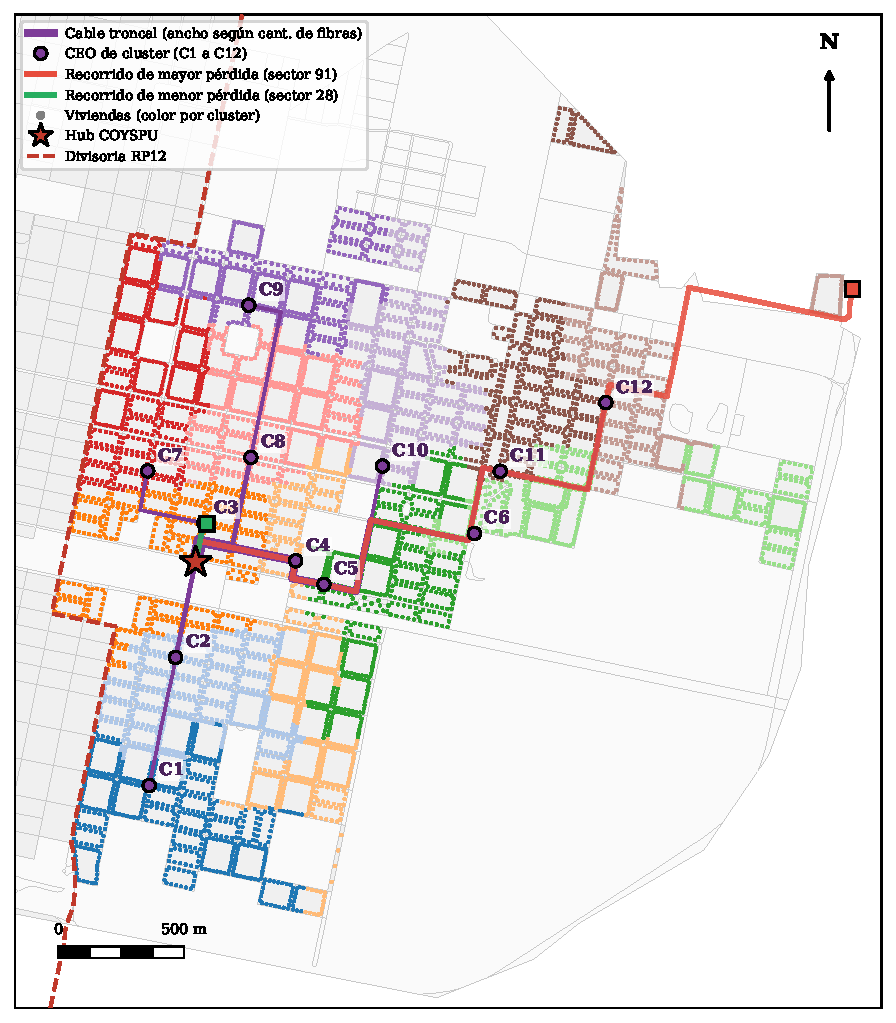
\includegraphics[width=0.95\textwidth]{plano_este_troncal.pdf}
    \caption{Región Este: traza del cable troncal, cajas de empalme de cluster y recorridos de mayor y menor pérdida óptica.}
    \label{fig:troncal}
\end{figure}

\footnotesize\setlength{\tabcolsep}{4pt}\begin{longtable}{|c|l|l|r|r|c|p{4.2cm}|}
\caption{Tramos del cable troncal de la Región Este.}\label{tab:tramos}\\ \hline
\textbf{Tramo} & \textbf{Desde} & \textbf{Hasta} & \textbf{L [m]} & \textbf{Fibras} & \textbf{Cable} & \textbf{Recorrido (calles)} \\ \hline \endfirsthead
\hline \textbf{Tramo} & \textbf{Desde} & \textbf{Hasta} & \textbf{L [m]} & \textbf{Fibras} & \textbf{Cable} & \textbf{Recorrido (calles)} \\ \hline \endhead
CT-01 & Hub COYSPU & D1 & 5 & 240 & 2x144F & 9 de Julio \\ \hline
CT-02 & Hub COYSPU & CEO-C2 & 388 & 48 & 1x48F & 9 de Julio, Perú \\ \hline
CT-03 & D1 & D2 & 128 & 144 & 1x144F & Boulevard Lardizabal \\ \hline
CT-04 & D1 & CEO-C3 & 153 & 72 & 1x72F & 9 de Julio \\ \hline
CT-05 & D1 & CEO-C7 & 569 & 24 & 1x24F & Avenida San Martín, Boulevard Lardizabal, Italia \\ \hline
CT-06 & D2 & CEO-C4 & 340 & 48 & 1x48F & Justo José de Urquiza, Pasaje Maipú \\ \hline
CT-07 & D2 & CEO-C5 & 398 & 96 & 1x96F & Boulevard Lardizabal, Jujuy \\ \hline
CT-08 & CEO-C3 & D3 & 144 & 48 & 1x48F & 9 de Julio \\ \hline
CT-09 & D3 & CEO-C8 & 277 & 24 & 1x24F & Avenida Belgrano, Justo José de Urquiza \\ \hline
CT-10 & D3 & CEO-C9 & 851 & 24 & 1x24F & 9 de Julio \\ \hline
CT-11 & CEO-C2 & CEO-C1 & 521 & 24 & 1x24F & Perú \\ \hline
CT-12 & CEO-C4 & CEO-C10 & 695 & 24 & 1x24F & Avenida Belgrano, Bismark, Boulevard Hipólito Irigoyen \\ \hline
CT-13 & CEO-C5 & D4 & 270 & 72 & 1x72F & Avenida San Martín, Garibaldi \\ \hline
CT-14 & D4 & CEO-C6 & 590 & 48 & 1x48F & Avenida San Martín, Fuerza Aérea Argentina, Los Robles \\ \hline
CT-15 & D4 & CEO-C11 & 898 & 24 & 1x24F & Avenida Roque Sanz Peña Este, Bismark, Boulevard Roque Sáenz Peña \\ \hline
CT-16 & CEO-C6 & CEO-C12 & 994 & 24 & 1x24F & Avenida Belgrano, Avenida Roque Sanz Peña Este, Hermanas Vicentinas \\ \hline
\multicolumn{3}{|r|}{\textbf{Total de traza}} & \textbf{7.222} & \multicolumn{3}{l|}{} \\ \hline
\end{longtable}

\begin{table}[H]\centering\footnotesize
\caption{Ubicación de las cajas de empalme del troncal.}\label{tab:nodos}
\begin{tabular}{|l|l|}\hline \textbf{Identificación} & \textbf{Ubicación (intersección de calles)} \\ \hline
Hub COYSPU & 9 de Julio 99 (Cooperativa COYSPU) \\ \hline
CEO-C1 & Avenida Zeballos y Perú \\ \hline
CEO-C2 & 3 de Febrero y Perú \\ \hline
CEO-C3 & 9 de Julio y Avenida San Martín \\ \hline
CEO-C4 & Champagnat y Pasaje Maipú \\ \hline
CEO-C5 & Boulevard Lardizabal y Garibaldi \\ \hline
CEO-C6 & Los Robles \\ \hline
CEO-C7 & Leandro N. Alem \\ \hline
CEO-C8 & Boulevard Hipólito Irigoyen y Justo José de Urquiza \\ \hline
CEO-C9 & 9 de Julio y Avenida Rivadavia \\ \hline
CEO-C10 & Bismark y O'Higgins \\ \hline
CEO-C11 & Avenida Roque Sanz Peña Este y Timoteo Gordillo \\ \hline
CEO-C12 & Hermanas Vicentinas y Pasaje Juan Cruz González Este \\ \hline
D1 & 9 de Julio y Boulevard Lardizabal \\ \hline
D2 & Boulevard Lardizabal y Justo José de Urquiza \\ \hline
D3 & 9 de Julio y Avenida Belgrano \\ \hline
D4 & Avenida San Martín y Bismark \\ \hline
\end{tabular}\end{table}


\textbf{Ubicación de cajas y splitters:}
\begin{itemize}
    \item \underline{Cajas de empalme del troncal (FK-CEO-4M):} en las 12 CEO de cluster y en los 4 puntos de derivación D1 a D4 (\autoref{tab:nodos}), donde cambia la capacidad del cable.
    \item \underline{Cajas de distribución (FK-CEO-4M con splitter 1:4):} una por sector (92 en total), en la esquina que minimiza el recorrido de distribución hasta sus CTO. Su ubicación se lista en el \autoref{anexo:sectores}.
    \item \underline{Cajas terminales (FK-CTO-16MC con splitter 1:16):} 365 cajas en postes de esquina, cada una para hasta 17 viviendas.
\end{itemize}

\textbf{Reservas de cable:} se deja un rulo de reserva de $20 \, [m]$ en cada CEO y caja de distribución y de $10 \, [m]$ en cada CTO. Esto permite reabrir los empalmes y reubicar las cajas sin reemplazar el cable. Además, se adiciona un 10\,\% a las longitudes de traza por catenaria, bajadas y desvíos en los postes.

\subsubsection{Aspectos que requieren verificación de campo}
\label{sec:verificacion}
\begin{itemize}
    \item \underline{Postería:} propiedad, estado, altura y vanos reales, y acuerdo de uso con su propietario (la COYSPU no figura como distribuidora eléctrica \cite{coyspu}, por lo que el permiso debe gestionarse con la distribuidora o el municipio).
    \item \underline{Cruces especiales:} cruces de la RN9, de la RP12 y de la traza ferroviaria, que pueden requerir tendido subterráneo o permisos de Vialidad y del concesionario ferroviario.
    \item \underline{Viviendas reales:} cantidad de viviendas por manzana, en especial en el centro, donde los edificios de departamentos requieren un diseño vertical propio, y en los barrios en expansión de la periferia, donde OpenStreetMap puede no estar actualizado.
    \item \underline{Calles sin nombre y loteos nuevos} en el noreste de la región (sectores 91 y 92).
    \item \underline{Ubicación exacta del nodo REFEFO} y de la red de fibra existente de la COYSPU, que podría reutilizarse para el enlace mayorista.
\end{itemize}

\subsection{Desarrollo de dos sectores}
\label{sec:sectores}
Se desarrollan en detalle dos sectores representativos:
\begin{itemize}
    \item El \textbf{sector 28} (cluster C3), en el centro, junto al hub, que contiene el recorrido de menor pérdida de la región.
    \item El \textbf{sector 90} (cluster C12), en la periferia noreste: es el sector completo, con 4 CTO, más alejado del hub.
\end{itemize}

En ambos casos las fibras del cable de distribución de 12 fibras se asignan así:
\begin{itemize}
    \item F1 a F4: salidas 1 a 4 del splitter 1:4, una para cada CTO.
    \item F5 a F8: crecimiento.
    \item F9 a F12: reserva.
\end{itemize}
En cada CTO, el splitter 1:16 conectorizado tiene sus salidas numeradas del 1 al 16, y cada salida corresponde a una vivienda.

\subsubsection{Sector 28}
El sector 28 tiene 67 viviendas en las manzanas comprendidas entre 9 de Julio, Av. San Martín, Av. Belgrano y Pasaje Maipú (\autoref{fig:sector28}). Su caja de distribución CD-28 está en 9 de Julio y Av. San Martín, en el mismo poste que la CEO del cluster C3, por lo que ambas funciones pueden resolverse en una única caja FK-CEO-4M. El cable de distribución mide $230 \, [m]$ y la acometida más larga es de $109 \, [m]$ (\autoref{tab:sector28}).

\begin{figure}[H]
    \centering
    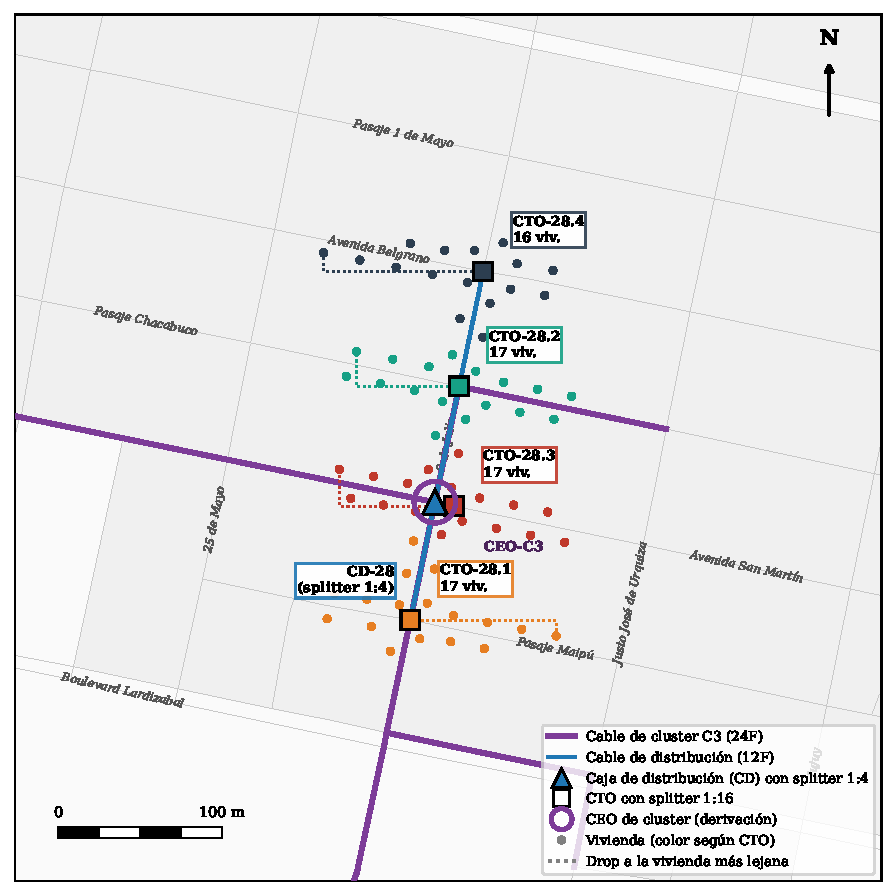
\includegraphics[width=0.85\textwidth]{plano_sector_28.pdf}
    \caption{Plano ampliado del sector 28 (cluster C3).}
    \label{fig:sector28}
\end{figure}

\begin{table}[H]\centering\footnotesize
\caption{Cajas terminales del sector 28 (cluster C3).}\label{tab:sector28}
\begin{tabular}{|c|p{4.0cm}|r|r|r|c|}\hline \textbf{CTO} & \textbf{Ubicación} & \textbf{Viv.} & \textbf{Desde CD [m]} & \textbf{Drop máx. [m]} & \textbf{Fibra/salida} \\ \hline
CTO-28.1 & 9 de Julio y Pasaje Maipú & 17 & 74 & 99 & F1 / 1 \\ \hline
CTO-28.2 & 9 de Julio y Pasaje Chacabuco & 17 & 72 & 84 & F2 / 2 \\ \hline
CTO-28.3 & Avenida San Martín & 17 & 12 & 93 & F3 / 3 \\ \hline
CTO-28.4 & 9 de Julio y Avenida Belgrano & 16 & 144 & 109 & F4 / 4 \\ \hline
\end{tabular}\end{table}


\subsubsection{Sector 90}
El sector 90 tiene 67 viviendas en el noreste de la región, alrededor de Hermanas Vicentinas y Soberanía Nacional Este (\autoref{fig:sector90}). Su caja de distribución CD-90 está en Hermanas Vicentinas y Soberanía Nacional Este, a $2{,}92 \, [km]$ del hub por el troncal y el cable de cluster. Por la menor densidad de viviendas, el cable de distribución es más largo ($633 \, [m]$) y la acometida más larga alcanza $227 \, [m]$ (\autoref{tab:sector90}). Es aceptable para un drop autosoportado, pero la ubicación de la CTO-90.4 debe revisarse en campo para acortarla.

\begin{figure}[H]
    \centering
    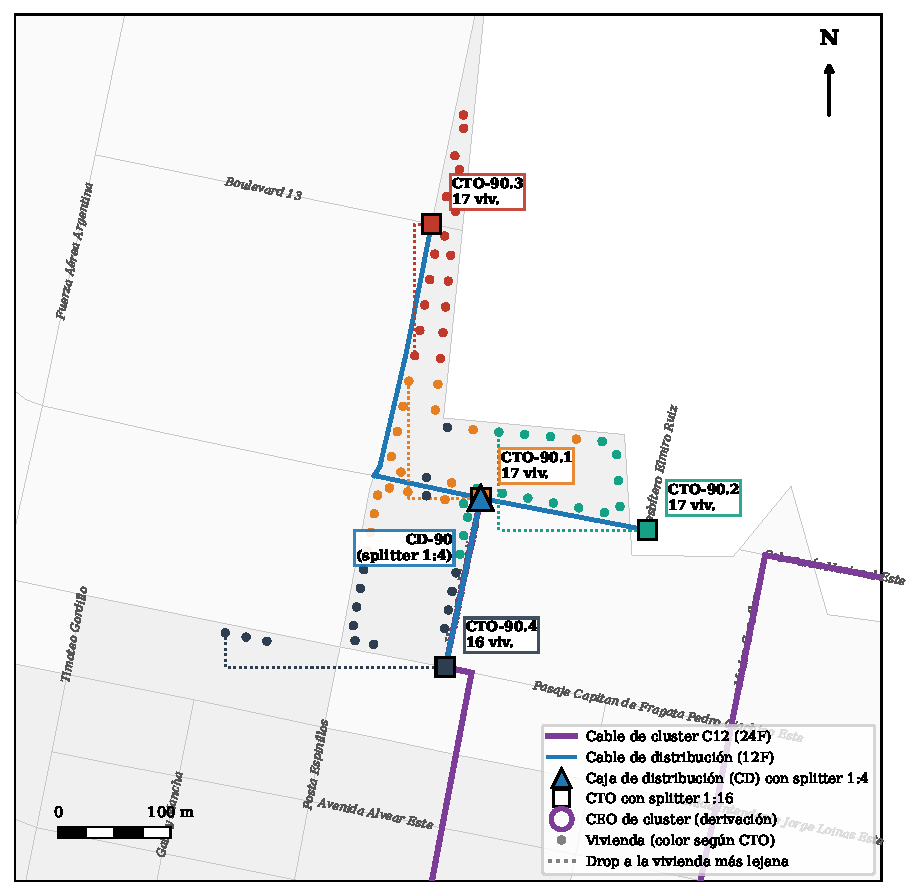
\includegraphics[width=0.85\textwidth]{plano_sector_90.pdf}
    \caption{Plano ampliado del sector 90 (cluster C12).}
    \label{fig:sector90}
\end{figure}

\begin{table}[H]\centering\footnotesize
\caption{Cajas terminales del sector 90 (cluster C12).}\label{tab:sector90}
\begin{tabular}{|c|p{4.0cm}|r|r|r|c|}\hline \textbf{CTO} & \textbf{Ubicación} & \textbf{Viv.} & \textbf{Desde CD [m]} & \textbf{Drop máx. [m]} & \textbf{Fibra/salida} \\ \hline
CTO-90.1 & Hermanas Vicentinas y Soberanía Nacional Este & 17 & 0 & 169 & F1 / 1 \\ \hline
CTO-90.2 & Presbítero Elmiro Ruiz y Soberanía Nacional Este & 17 & 151 & 220 & F2 / 2 \\ \hline
CTO-90.3 & Boulevard 13 y Posta Espinillos & 17 & 328 & 132 & F3 / 3 \\ \hline
CTO-90.4 & Hermanas Vicentinas y Pasaje Capitan de Fragata Pedro Giachino Este & 16 & 154 & 227 & F4 / 4 \\ \hline
\end{tabular}\end{table}


\pendiente{Región Oeste: organización en clusters y sectores, trazas y desarrollo de sus dos sectores, a cargo de Mendes Rosa y Monja.}
